\RequirePackage{fix-cm}
\documentclass[11pt]{article}
\usepackage[fontsize=12pt]{scrextend}
\usepackage{geometry} 
\usepackage{graphicx}
\usepackage{url}
\usepackage{mathtools}
\usepackage{amsmath}
\usepackage{amsfonts}
\usepackage{bigints}
\usepackage{soul,color}
\usepackage{epigraph}
\usepackage[super,numbers,sort&compress]{natbib}
\usepackage[font=scriptsize,labelfont=bf]{caption}
\usepackage[parfill]{parskip}
\usepackage{wrapfig}
%\usepackage{pgfgantt}
\usepackage[hidelinks]{hyperref}
\parskip=8pt
\pagenumbering{gobble}

\bibliographystyle{plos2015}

\geometry{
a4paper,
top=1in,
left=1in,
right=1in,
bottom=1in
} 

\setlength{\parindent}{1.5em}
\setlength{\parskip}{0.1em}

\newcommand{\gb}[1]{{\color{blue}{#1}}}

%	 NOTES ON PROPOSAL
%            1-2pg pre-proposal that includes:
%		general budget
%		relevant personnel (Peter, Gideon, a pdoc tbd)
%		approach
%		deliverables (density, movement, xvalidation w/ previous years/findings)
%			timeline
%		dataset will consist of ~150-200 SNPs


\begin{document}
%
\begin{center}
\textbf{Developing a close-kin mark-recapture model to map black bear population numbers in Michigan's Upper Peninsula}
\end{center}
%            
\vspace{0.5em}

\noindent Dr.~Gideon Bradburd, Dept.~of Integrative Biology, Michigan State University\\
\noindent Dr.~Peter Ralph, Depts.~of Mathematics and Biology, University of Oregon

\vspace{1em}

\noindent
Accurate population size estimates 
for managed or threatened species  
are vital for implementing informed management strategies.
In Michigan, black bears (\textit{Ursus americanus}) 
are managed by harvesting, 
and estimates of the population size are used in determining
the hunting license quota.
Accurate, up-to-date estimates of 
the bear population size in the state 
-- ideally, by age and by region --
are therefore a necessary component 
of any effective management plan.

Recent bear population monitoring efforts 
in the state of Michigan have relied on 
capture-mark-recapture (CMR) methods, 
by which a sample of a population is initially marked, 
and an estimate of total population abundance 
can be made from the number of marked individuals 
that are subsequently recaptured (or harvested). 
However, traditional CMR methods are not ideal:  
they require extra fieldwork to do initial population marking; 
the tetracycline biomarker used in marking black bear individuals is no longer permitted; 
and there is a substantial wait time (1-3 years) after the 
initial marking period until population estimates can be made.
Statistical catch-at-age analysis (SCAA)
fits a demographic model to age and fecundity distributions
estimated from harvested bears,
thus allowing population size estimation without costly and time-intensive
fieldwork \citep{mayhew2019}.
However, since SCAA does not directly estimate absolute population size,
to remain accurate it needs periodic recalibration with another method, e.g., CMR.

\begin{wrapfigure}{r}{.4\textwidth}
    \centering
      \vskip -1em
        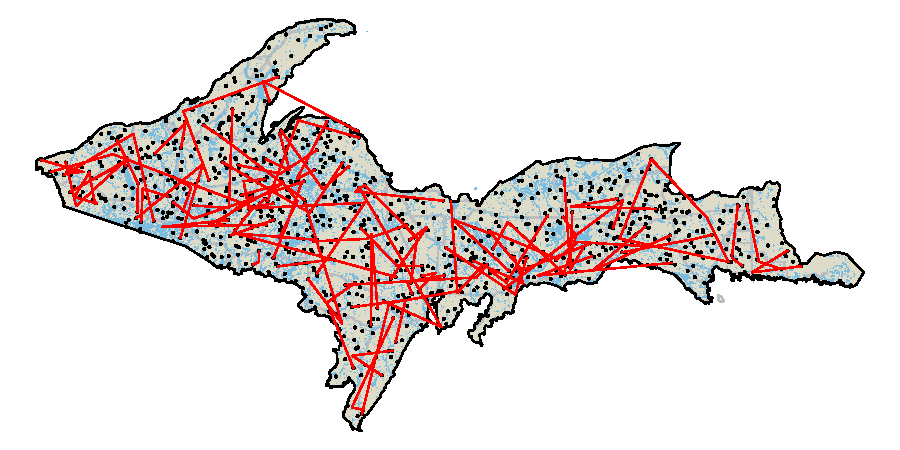
\includegraphics[width=.4\textwidth]{{../sims/bears_K1.0.bear_sibs}.pdf}
        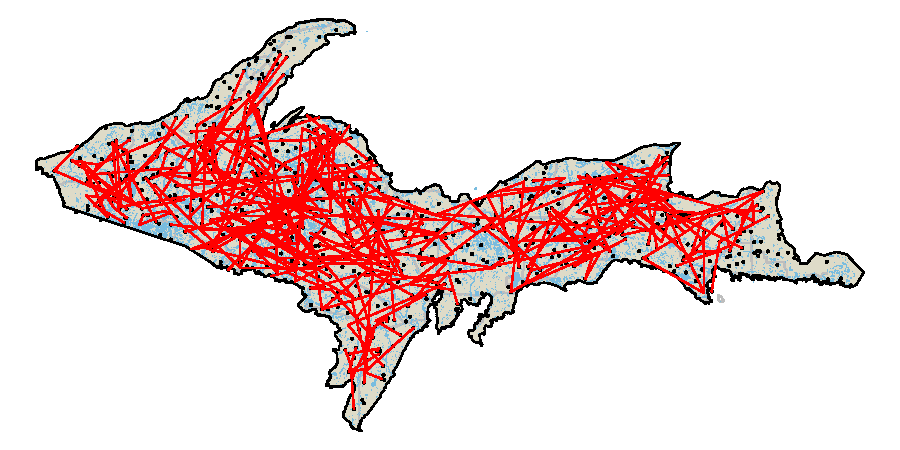
\includegraphics[width=.4\textwidth]{{../sims/bears_K0.25.bear_sibs}.pdf}
    \caption{  \label{fig:maps}
    Locations of sampled bears (black points)
    and relationships of sampled half-sibs (red lines),
    in spatially explicit simulations of sexual, age-structured populations
    with local density-dependent population regulation,
    at two values of local population density.
    In the top figure, a total population of around 14,000 bears resulted in
    73 half-sib pairs out of 1,000 harvested bears,
    while in the lower figure, a smaller total population of around 3,300 resulted in
    216 half-sib pairs out of the same harvested number.
    }
\end{wrapfigure}

Genetic data from sampled individuals can be used to produce
an accurate and cost-effective alternative to CMR 
for estimating population sizes \citep{Skaug2001,Hettiarachchige2018}. 
Genetic mark-capture methods use 
an individual's genetic data in lieu of
the initial marking phase in a standard CMR,  
and may therefore use 
data collected solely from harvested animals.

Close-kin mark-recapture (CKMR) models 
are an exciting class of genetic mark-recapture methods 
that leverage advances in molecular genetics 
to estimate population size 
from kinship patterns inferred in a genotyped sample 
\citep{bravington2016closekin,ruzzante2019validation}.
To build an intuition for how relatedness 
between sampled individuals can be informative 
about total population size, 
we can consider the number of siblings in a sample.
As depicted in Figure~\ref{fig:maps},
a random sample from a population 
with a small number of breeding adults 
is more likely to contain siblings than that 
from a population with a large number of breeding adults; 
the number of sibling-pairs of various ages in a sample can 
therefore be used to infer the recent history of adult population sizes.

CKMR approaches offer a number of advantages 
over competing models. 
Like all genetic mark recapture models, 
a CKMR approach requires only a single round of sampling, 
which can be achieved through a harvest.
(It would be more accurate to refer to CKMR as 
a Close-Kin Capture method, 
as there is no marking phase, 
so it therefore requires no recapture.)
These methods also avoid some types of bias 
that can be introduced into CMR methods due to 
heterogeneity in capture/recapture probability.
Moreover, by focusing on multiple pedigree connections 
(e.g., half-sib relationships, 
in addition to parent-offspring and full-sib) 
they allow a researcher to study unsampled individuals.

Here, we propose to develop a CKMR model 
for black bears in Michigan's Upper Peninsula (UP) 
for use by the Michigan Department of Natural Resources.
This model, which will account for 
variable fecundity and capture probability, 
as well as non-sparse and non-uniform sampling, 
will generate population size estimates 
for the adult, pre-harvest black bear population in the UP. 
Because spatial structure in the bear population might impact 
population size estimates, 
we will also extend existing CKMR models 
to incorporate geography.
In addition to generating estimates of total population size 
that are robust to the spatial structure of the pedigree, 
this spatial model will also generate maps of estimated 
population density, 
and has the potential to shed light 
on other demographic parameters as well.
This model will be extensively tested using spatially explicit,  
forward-time simulations. 
To demonstrate the feasibility of this approach, 
we have included preliminary simulations 
of the bear population in the UP (Fig \ref{fig:maps}).
These simulations, 
which were run with SLiM \citep{haller2018forward},
output both whole-genome genotypes and actual genealogical relationships,
and have many realistic demographic features 
(e.g., nonuniform density and local post-natal dispersal) 
but are only proof-of-concept
(code available at \url{https://github.com/petrelharp/howmanybears}).
Biological parameters used to simulate these tests  
will be informed by previous 
research on Michigan black bears \citep{moore2014application, mayhew2019} and partner feedback.
These simulations will be used both to 
validate the proposed inference procedure 
and to explore the sensitivity of the output to model assumptions 
(all model assumptions will be listed in the model documentation).

To disseminate the results of this new model, 
we will implement it in well-documented scripts 
that produce templated reports and graphical output
for easy use by the DNR, 
and provide accompanying vignettes 
and a video walk-through demonstration. 
We will also engage in educational trainings with state biologists, 
and assist in outreach with 
administrators, commissioners, and stakeholders.

We are confident that we will be able to 
carry out the proposed work in the timeline below (Fig \ref{timeline}).
Both PIs Bradburd and Ralph have extensive 
experience developing statistical methods \citep{bedassle, SpaceMix, bradburd2018inferring} -- 
with a particular focus on spatial population genetics \citep{bradburd2019spatial, Battey_etal_2020} -- 
and implementing them as documented software packages.
In addition, the PIs have collaborated previously 
on black bear research \citep{bradburd2018inferring}
and on developing management plans 
for government agencies \citep{shaffer2017desert}, 
and have recently co-written a review discussing how to link properties of the pedigree
to population demography and dynamics \citep{bradburd2019spatial}.
% value added: all inds simultaneously vs. one dyad at a time? ; MI-specifc simulation framework

\begin{figure}[h!]
    \centering
         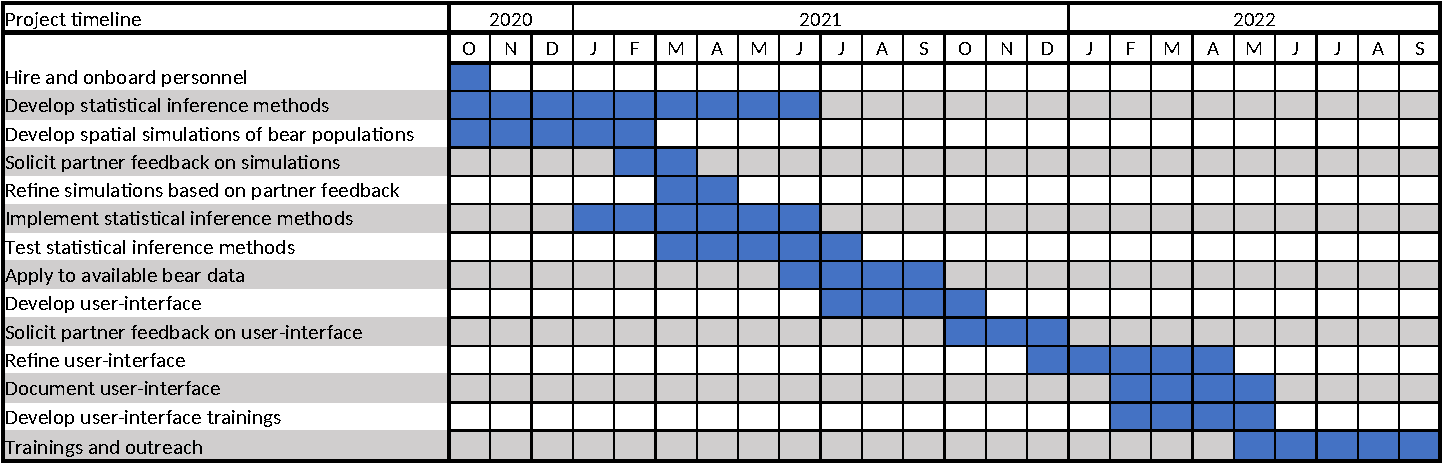
\includegraphics[width=0.92\linewidth]{bear_gantt_chart.pdf}
		\vspace{-0.5em}
        \caption{
		Timeline of proposed work.
        }
        \label{timeline}
\end{figure}

\clearpage
\bibliography{references.bib}
\end{document}
